\documentclass[12pt]{book}
\usepackage[dvips,xetex]{graphicx}
\usepackage[margin=1in]{geometry} 
\geometry{a4paper}
\graphicspath{{images/}}
\usepackage{titling}
\usepackage[T1]{fontenc}
\usepackage[utf8]{inputenc}
\usepackage{lmodern}
\usepackage{color}
\usepackage{xepersian}

\settextfont{IRANSans}
\title{\textbf{خودآموز زبان C}}

%\author{نوشته شده توسط\\ \textbf{سعید}\\ \small \color{red}pymancore@riseup.net}

\begin{document}
\begin{figure}
\centering
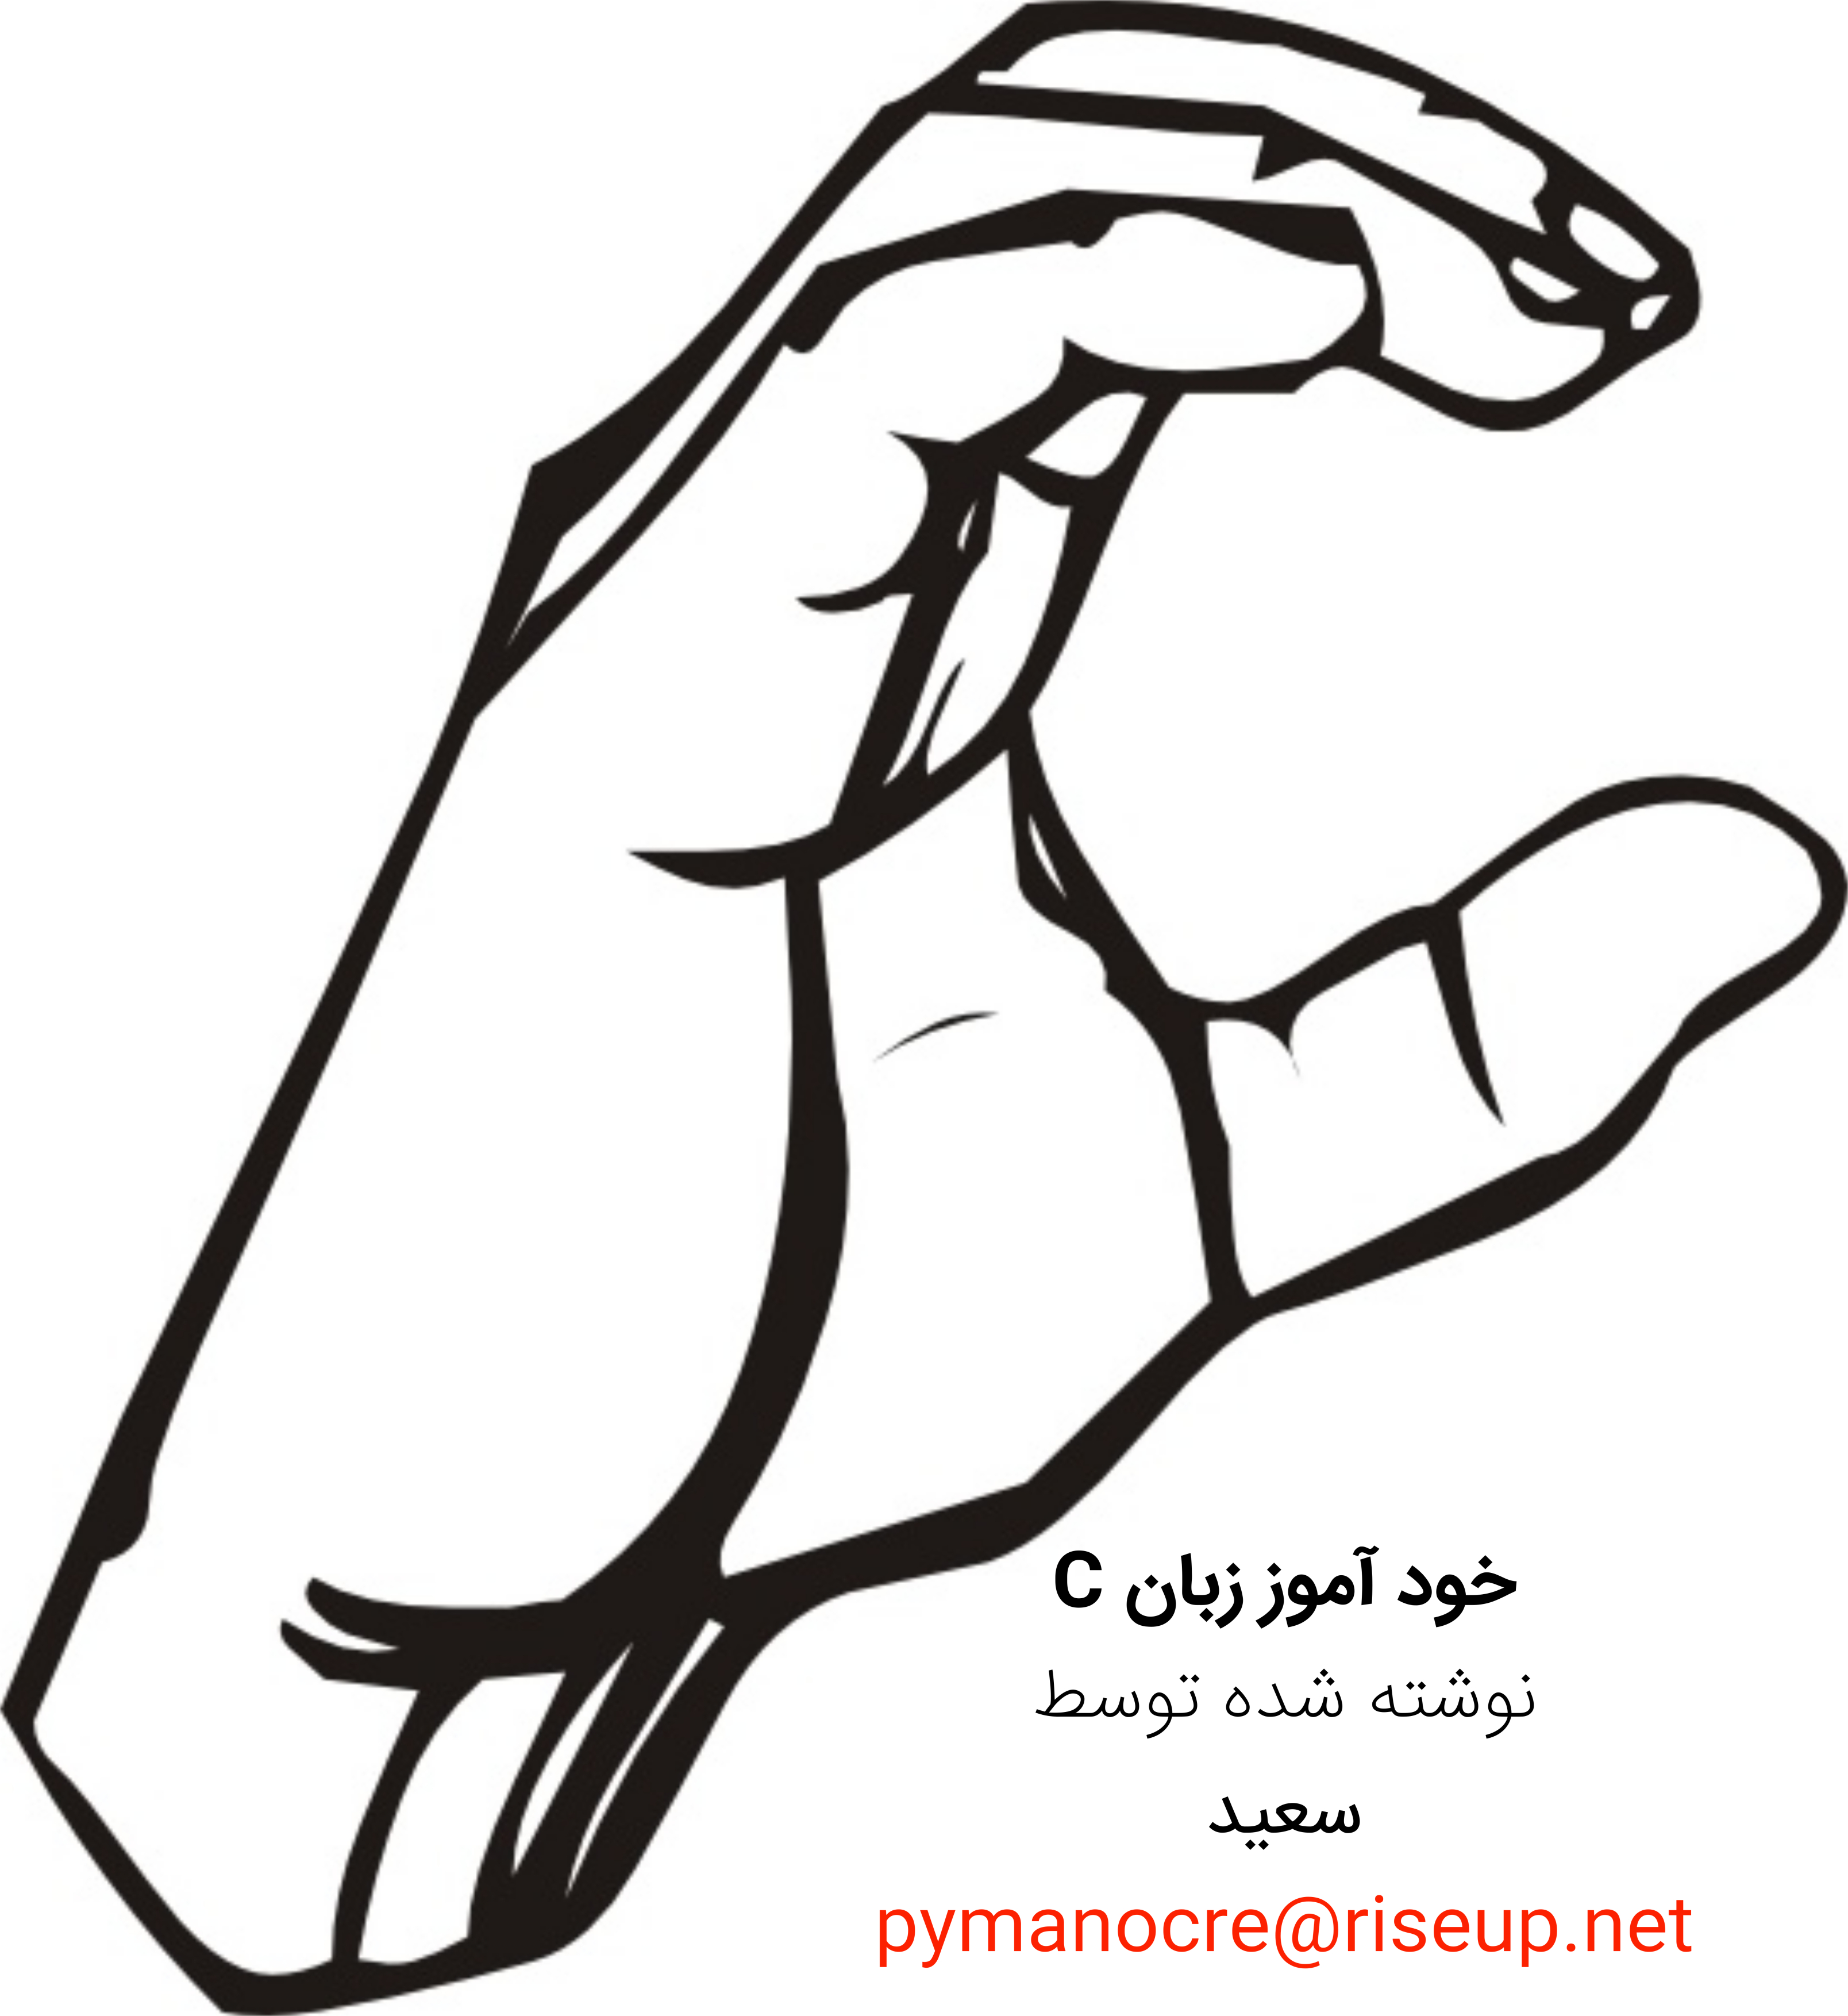
\includegraphics[width=170mm]{c_artwork}
\end{figure}
\maketitle

\tableofcontents
\addcontentsline{toc}{chapter}{پیش‌گفتار}
\chapter*{پیش‌گفتار}
  در اینجا ما امتحان میکنیم.

\part{مفاهیم و تعاریف}
\chapter{تعریف برنامه‌نویسی}
\section{برنامه‌نویسی و زبان برنامه‌نویسی}
\section{برنامه و اسکریپت}

\chapter{تاریخچه زبان C}

\chapter{استاندارهای C}
\section{استاندارد ANSI/ISO}
\section{استاندارد C99}
\section{استاندارد C11}
\section{استاندارد C18}

\chapter{ویژگی‌های زبان C}
\section{طراحی}
\subsection{ساختار بالا به پایین}
\subsection{کتابخانه‌های استاندارد}
\subsection{برنامه‌نویسی ماژولار}
\section{بهینگی}
\section{قابلیت حمل}
\section{قدرت و انعطاف‌پذیری}
\section{آزادی}

\end{document}
